\documentclass[10pt]{article}
\usepackage[margin=1in]{geometry}
\usepackage[T1]{fontenc}
\usepackage{amsmath,amssymb,booktabs,graphicx,xurl}
\usepackage[hidelinks]{hyperref}
\usepackage{microtype}
\title{Does Predicting Chess Transitions Improve Small Recurrent Policies?}
\author{OpenJev project}
\date{Development study, September 2026}
% Generated from the audited completed release.
\newcommand{\PredictDev}{32.97}
\newcommand{\PredictShift}{25.43}
\newcommand{\ReconstructDev}{32.69}
\newcommand{\ReconstructShift}{25.22}
\newcommand{\GateOutcome}{did not meet its descriptive development threshold}
\newcommand{\ResultInterpretation}{The results do not establish that future prediction improves decisions over the controls.}
\newcommand{\ResultDiscussion}{Prediction minus reconstruction teacher agreement is +0.28 percentage points on ordinary development and +0.21 points under the specified shift. All twelve final fits are retained. No best seed or checkpoint is selected. Auxiliary accuracy and policy quality answer different questions.}
\newcommand{\TrainingMinutes}{3.04}

\begin{document}
\maketitle
\begin{abstract}
We test whether action-conditioned prediction of future board pieces improves a
small chess policy beyond equally expensive reconstruction of current pieces.
A shared spatial candidate scorer avoids a separate classifier for every move.
Three recurrent variants share architecture, initialization and training budgets;
an untied convolutional network supplies a further spatial baseline.
Twelve final fits use 32,768 freshly generated Stockfish-labeled positions and
are evaluated on 4,096 ordinary and 4,096 shifted development positions.
The prediction model obtains \PredictDev\% and \PredictShift\% mean teacher
agreement, compared with \ReconstructDev\% and \ReconstructShift\% for
reconstruction. The predeclared continuation criterion \GateOutcome.
\ResultInterpretation{}
This is a development experiment, not an Elo estimate, novel planning algorithm,
biological-connectome result or claim of submission readiness.
\end{abstract}

\section{Motivation and related work}
The first OpenJev chess study tested a synthetic signed recurrent circuit against
a degree-preserving rewired control and a GRU. Mean teacher agreement was about
14\%; the topology criterion failed. A subsequent diagnostic on already scored
data showed weak sensitivity to shuffled board features and a 16-coordinate
input bottleneck in the circuit. These observations motivated better spatial
representations before additional topology claims. That diagnosis is post-hoc;
the present study excludes every position from that earlier training and
development set, including color-mirrored equivalents.

Recurrence on chess, including additional inference iterations, is established
by Schwarzschild et al.~\cite{schwarzschild2021}. Stockfish policy and value
distillation are established, including comparisons between behavioral cloning,
state-value and action-value targets in ChessBench~\cite{ruoss2024}.
Action-conditioned learned dynamics used for planning are established by
MuZero~\cite{schrittwieser2020}. Our specific question is whether transition
supervision adds useful information beyond an equally expensive reconstruction
objective in a small legal-candidate policy. This comparison does not by itself
establish a new algorithm.

\section{Model and controlled intervention}
\subsection{Spatial state and legal candidates}
We encode a board as $x\in\mathbb{R}^{19\times8\times8}$. Twelve piece planes
identify own and opposing pieces. Four constant planes encode castling rights,
one plane marks the recorded en-passant square, and two constant planes encode
move counters. Black-to-move boards are rank-mirrored and ownership is relative
to the mover. python-chess supplies all legal moves. No SAN check/mate annotations,
teacher scores or target moves are included in model inputs.

A 32-channel convolutional encoder produces $h^{(0)}$. The recurrent models apply
one two-convolution residual block four times:
\begin{equation}
 h^{(k+1)}=\operatorname{ReLU}\!\left(h^{(k)}+
 W_2*\operatorname{ReLU}(W_1*h^{(k)}+b_1)+b_2\right).
\end{equation}
A single head scores each legal move $a=(s,t,p)$ from source-square features,
destination-square features, mean-pooled board features, and learned embeddings
of promotion and displacement:
\begin{equation}
 \ell_a=f_\theta\!\left(h_s^{(4)},h_t^{(4)},\bar h^{(4)},e_p,e_{\Delta x},e_{\Delta y}\right),
 \qquad \pi(a\mid x)=\frac{\exp\ell_a}{\sum_{b\in\mathcal A(x)}\exp\ell_b}.
\end{equation}
The value head is a bounded scalar. Softmax scores are uncalibrated candidate
probabilities; the value target is not a win probability. State resets for every
board, with no persistent game memory or inference search.

\subsection{Auxiliary transition prediction}
Four fixed uniformly sampled distinct legal actions per position, or all actions
if fewer exist, produce exact successors through python-chess. A decoder receives
$h^{(4)}$ and source, destination and promotion planes for one action. It predicts
13 piece classes per square. Successor targets retain the \emph{pre-move}
perspective; changing side does not relabel or reflect the entire board.

Let $D(x,a)$ be squares whose piece class changes after the action. For squarewise
cross-entropy $c_i$, the auxiliary objective averages
\begin{equation}
 \mathcal L_{\mathrm{aux}}=\tfrac12\operatorname{mean}_{i\in D(x,a)}c_i+
                         \tfrac12\operatorname{mean}_{i\notin D(x,a)}c_i.
\end{equation}
Prediction uses successor pieces as labels; reconstruction uses current pieces.
Both use the same action inputs, changed-square masks, decoder and weight.
The no-auxiliary controls also execute and backpropagate through the branch,
with zero loss weight. Thus decoder operations are included in every training
budget. The full objective is
\begin{equation}
 \mathcal L= -\log\pi(a^*\mid x)+0.5(v_\theta(x)-\tanh(c/600))^2
               +\lambda\mathcal L_{\mathrm{aux}},
 \quad \lambda\in\{0,0.25\}.
\end{equation}

All recurrent variants have 43,726 parameters, including the auxiliary decoder.
An untied CNN starts with four independent copies of the same residual block,
with 99,214 parameters and the same number of executed blocks. Common initial
outputs match. CNN versus recurrent comparison changes parameter tying;
prediction versus reconstruction isolates the auxiliary target under the same
architecture and budget. The auxiliary decoder is not used to choose moves.
This is dynamics-supervised representation learning, not world-model planning.

\section{Frozen development protocol}
The public plan binds source hashes, dependencies, engine identity, exclusions,
seeds, game caps and optimization schedule before new data generation.
Stockfish 19 labels every visited nonterminal position using 2,000 requested
nodes, one thread, 16 MB hash and a cleared table. Labels receive the current FEN
without preceding history. Mate scores use python-chess's signed 10,000-centipawn
conversion, preserving mate distance. Rollout-only calls and actual reported
nodes are retained, not omitted from teacher cost.

Training and ordinary development mix uniform and teacher actions equally,
with a 64-ply cap. The shifted split uses 10\% uniform actions and a 96-ply cap.
Generated games are separate across splits. Global deduplication reserves piece
placement, side, castling and en-passant state, ignoring counters and merging
mirrored equivalents. This is a specified rollout-distribution shift, not a test
of broad environmental transfer.

Each arm uses seeds 17, 29 and 43; six epochs; batches of 128; Adam with learning
rate $10^{-3}$, betas $(0.9,0.999)$, epsilon $10^{-8}$, no weight decay; and gradient
norm clipping at 1. Same-seed batch orders match. Every fit receives 1,536 updates.
There is no early stopping, checkpoint selection, replacement fit or budget
extension. MPS training preserves data and initialization seeds but its indexing
gradients are not bitwise deterministic. All fits use the same device.

Untrained comparisons are exact uniform expectation, the most frequent training
UCI among legal moves, and a one-ply material heuristic. A fixed random subset of
128 positions per evaluation split receives an additional 20,000-node unrestricted
engine analysis and an equal-budget root-constrained analysis for every unique
chosen move. The reported bounded score difference is
$\tanh(c_{\rm unrestricted}/600)-\tanh(c_{\rm chosen}/600)$.
Finite searches can make it negative. It is a secondary engine estimate, not true
regret or a probability of losing. Identical choices share one engine call.

The continuation rule requires prediction to exceed every control by at least
two percentage points in mean teacher agreement in both splits, lose no more
than one point in any paired seed, and exceed 70\% changed-square prediction
accuracy. Both scored splits are development evidence. Passing this rule would
justify a fresh confirmation study, not an efficacy claim.

\section{Results}
\begin{table}[ht]
\centering\small
\begin{tabular}{lrrrrr}
\toprule
& & \multicolumn{2}{c}{Teacher agreement (\%)} & \multicolumn{2}{c}{Bounded engine difference} \\
Model & Parameters & Dev & Shift & Dev & Shift \\
\midrule
CNN & 99,214 & 33.02 & 25.33 & 0.108 & 0.137 \\
Recurrent & 43,726 & 32.90 & 25.58 & 0.103 & 0.120 \\
Reconstruct & 43,726 & 32.69 & 25.22 & 0.113 & 0.124 \\
Predict & 43,726 & 32.97 & 25.43 & 0.102 & 0.132 \\
\midrule
Material heuristic & 0 & 25.61 & 19.51 & 0.226 & 0.269 \\
\bottomrule
\end{tabular}
\caption{Mean of three fits for learned models. Higher agreement is better; lower bounded engine difference is better. Engine differences use 128 fixed positions per split and may be negative because searches are finite.}
\end{table}
\begin{table}[ht]
\centering\small
\begin{tabular}{llrrr}
\toprule
Model & Split & Changed squares (\%) & All squares (\%) & Exact boards (\%) \\
\midrule
Reconstruct & Dev & 0.69 & 93.64 & 0.00 \\
Reconstruct & Shift & 0.50 & 93.72 & 0.00 \\
Predict & Dev & 79.20 & 90.37 & 1.04 \\
Predict & Shift & 76.14 & 90.39 & 0.38 \\
\bottomrule
\end{tabular}
\caption{Decoder predictions assessed against actual successors. Reconstruction is trained to output current pieces, so this table is not an equal-objective reconstruction-quality comparison.}
\end{table}

\begin{figure}[t]
 \centering
 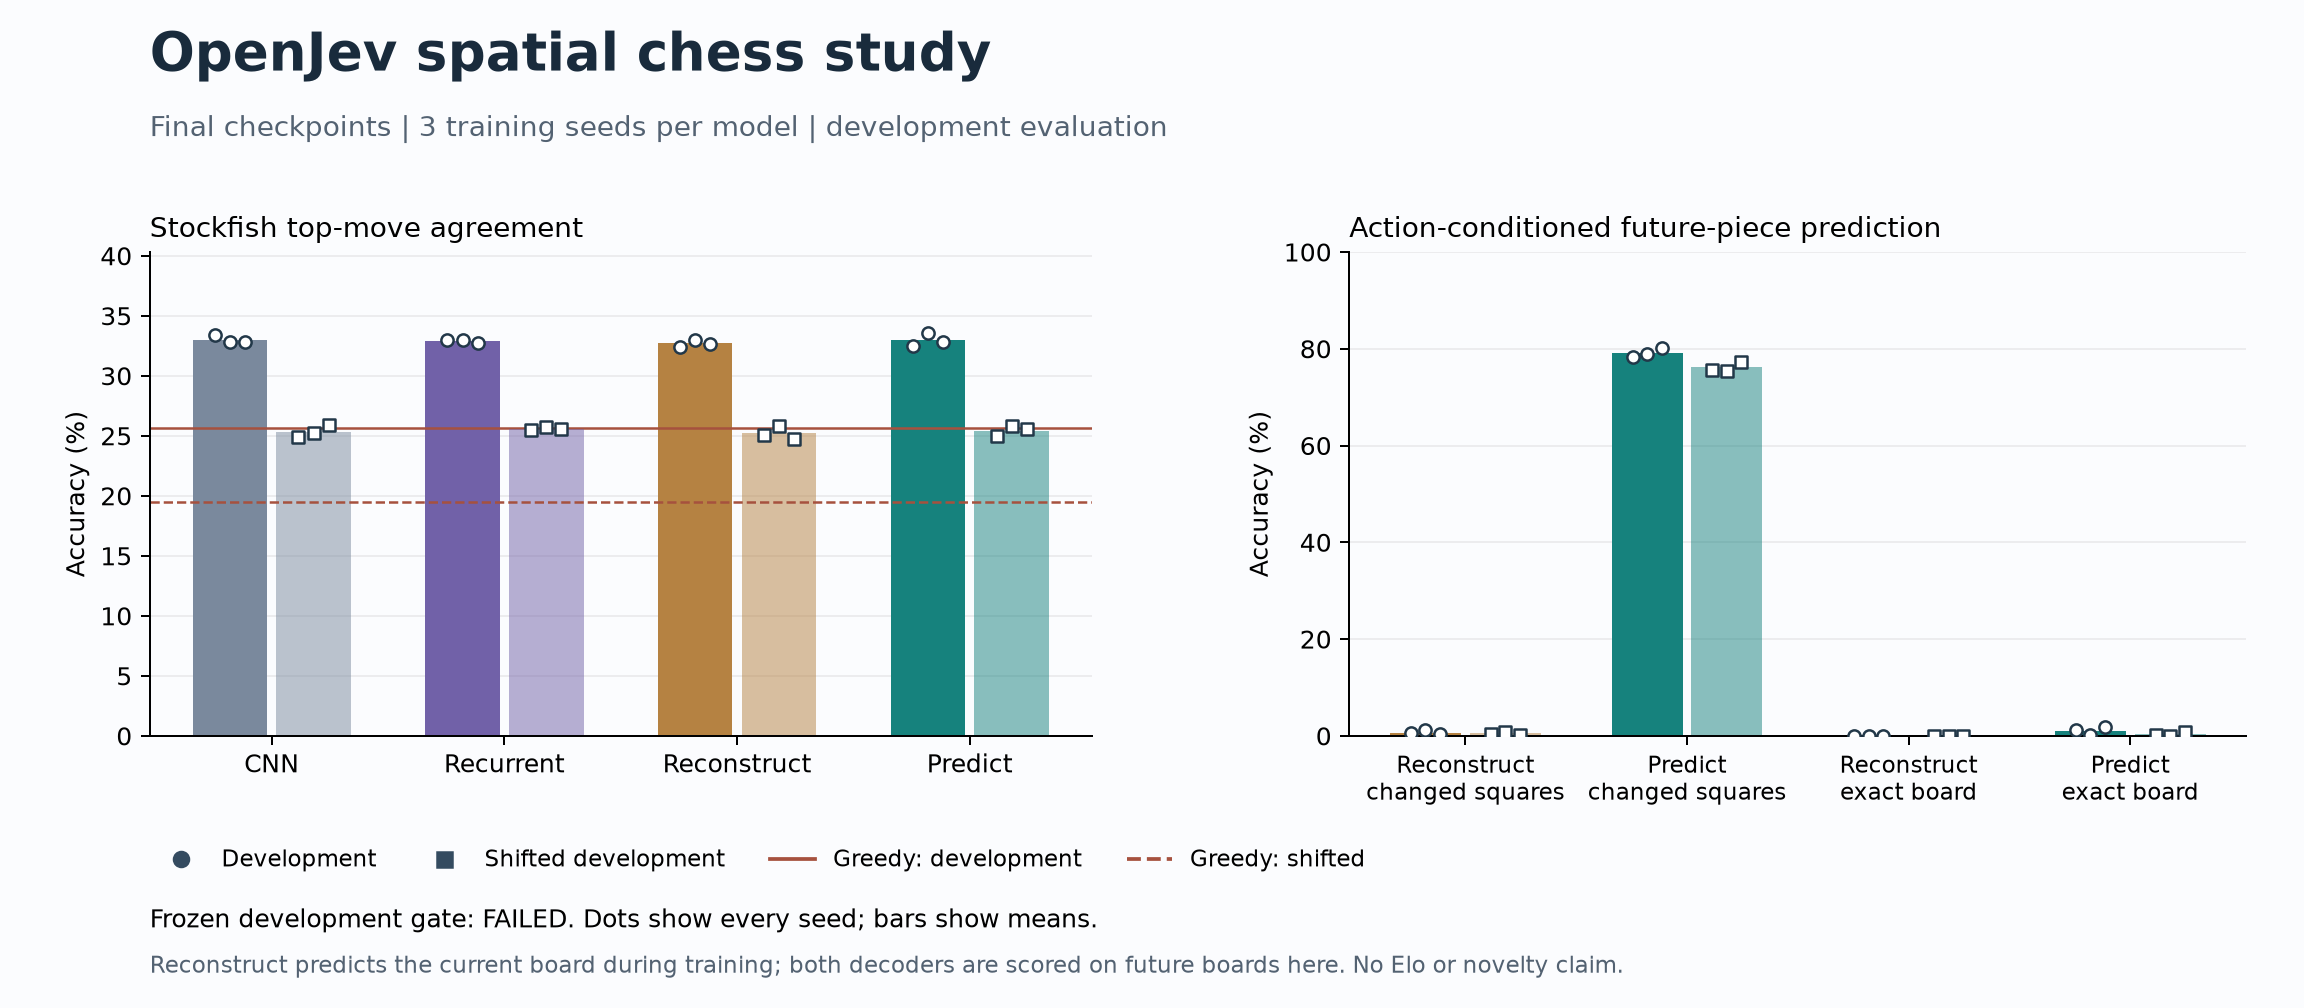
\includegraphics[width=\textwidth]{../docs/assets/chess-spatial-results.png}
 \caption{All final fits on the fixed development panels. Seed variation is
 visible; auxiliary prediction quality is distinguished from policy quality.
 Teacher agreement is not a gameplay win rate.}
\end{figure}

\ResultDiscussion

Copying unchanged squares is an inadequate dynamics baseline: changed-square
and exact-board accuracy are necessary alongside overall square accuracy.
The aggregate training time was \TrainingMinutes\ minutes; teacher generation,
evaluation, auxiliary target construction and secondary engine assessment are
separate costs. These wall times are local measurements, not a matched speed
comparison with external language models.

\section{Limits and next decision}
The study uses a single model width, fixed training schedule and three seeds.
Positions are correlated within games. Random/teacher rollout states may differ
substantially from human games. Teacher agreement treats different plausible
moves as errors and does not measure playing strength. The separate engine
assessment partially addresses that limitation with a small fixed subset.

Comparisons with the earlier flat student change both representation and data
budget, so they cannot isolate the contribution of spatial processing. The
within-study controls support the narrower comparisons. There is no new Astra,
ChessFly or ChessLFM score in this development panel. Prior heterogeneous games
and public puzzles remain separately reported.

Additional recurrent steps should first demonstrate a benefit under a fixed
budget before any learned computation gate is proposed. Any future latent
planning experiment must include exact successor-board scoring at matched cost:
chess already supplies a perfect symbolic transition simulator. A paper claiming
new computation allocation or learned planning would need a specific mechanism,
stronger controls, fresh confirmation and a second environment.

\paragraph{Artifacts.}
Code, frozen plans, every final checkpoint, raw data and all comparisons are
available in \url{https://github.com/kw2828/OpenJev}. Evidence is under
\texttt{evidence/chess-spatial-v1}; model weights are under
\texttt{models/chess-spatial-v1}. Original code and weights are MIT licensed;
external engine assets are not redistributed.

\begin{thebibliography}{9}
\bibitem{schwarzschild2021} A. Schwarzschild et al. Can You Learn an Algorithm?
Generalizing from Easy to Hard Problems with Recurrent Networks. NeurIPS, 2021.
\url{https://arxiv.org/abs/2106.04537}.
\bibitem{ruoss2024} A. Ruoss et al. Amortized Planning with Large-Scale Transformers:
A Case Study on Chess. 2024. \url{https://arxiv.org/abs/2402.04494}.
\bibitem{schrittwieser2020} J. Schrittwieser et al. Mastering Atari, Go, Chess and
Shogi by Planning with a Learned Model. Nature, 2020.
\url{https://arxiv.org/abs/1911.08265}.
\end{thebibliography}
\end{document}
